\documentclass{article}
\usepackage{tikz}
\usepackage{CJKutf8}
\usepackage{amsmath}
\usepackage{amsthm}
\begin{document}
\begin{CJK}{UTF8}{gbsn}
  \newtheorem*{Exercise}{习题}
  \huge
\begin{Exercise}[p314-3]
  有向图$D$的图解如下图所示:
  
  \centering
  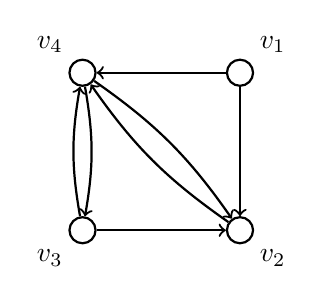
\begin{tikzpicture}[auto,
    specification/.style ={circle, draw, thick}]
   \node[specification] (A) [label=-135:$v_3$] at (0,0)  {};
   \node[specification] (B) [label=135:$v_4$] at (0,2)  {};
   \node[specification] (C) [label=45:$v_1$] at (2,2)  {};
   \node[specification] (D) [label=-45:$v_2$] at (2,0)  {};
   \draw[thick, ->] (A) to  (D);
   \draw[thick, ->] (C) to  (B);
   \draw[thick, ->] (C) to  (D);
   \draw[thick, ->] (A) to [bend left = 10] (B);
   \draw[thick, ->] (B) to [bend left = 10] (A);
   \draw[thick, ->] (B) to [bend left = 10] (D);
   \draw[thick, ->] (D) to [bend left = 10] (B);   
 \end{tikzpicture}\hspace{1cm}\\
 D

 \begin{enumerate}
  \renewcommand{\labelenumi}{(\theenumi)}
  \item 写出$D$的邻接矩阵及可达矩阵;
  \item 写出$D$的关联矩阵。
  \end{enumerate}
\end{Exercise}

\begin{proof}[解]
  D的邻接矩阵:\[\begin{bmatrix}0&1&0&1\\0&0&0&1\\0&1&0&1\\0&1&1&0\end{bmatrix}\]
  D的可达矩阵:\[\begin{bmatrix}1&1&1&1\\0&1&1&1\\0&1&1&1\\0&1&1&1\end{bmatrix}\]
  D的关联矩阵:\[\begin{bmatrix}1&1&0&0&0&0&0\\-1&0&0&-1&-1&0&1\\0&0&1&1&0&-1&0\\0&-1&-1&0&1&1&-1\end{bmatrix}\]
\end{proof}
\end{CJK}
\end{document}


%%% Local Variables:
%%% mode: latex
%%% TeX-master: t
%%% End:
